\chapter{Hasil Implementasi dan Pembahasan}

Bab ini menyajikan hasil implementasi dan pengujian sistem \textit{automated web penetration testing} berbasis \textit{Reinforcement Learning} yang telah dirancang pada Bab 3. Hasil yang diperoleh mencakup pengujian menggunakan algoritma Q-Learning dan Deep Q-Network (DQN) pada aplikasi target OWASP Juice Shop, serta perbandingan dengan \textit{scanner} konvensional OWASP ZAP. Analisis dilakukan berdasarkan metrik yang telah ditetapkan pada Bab 3, yaitu jumlah kerentanan yang ditemukan, tingkat deteksi, \textit{cumulative reward}, efisiensi jumlah \textit{request} per kerentanan, serta efektivitas \textit{payload} dan \textit{endpoint} yang diuji. Seluruh pembahasan mengacu pada data asli hasil pengujian yang tercantum pada \textit{file log}, \textit{summary}, dan laporan \textit{scanning} tanpa modifikasi atau rekayasa data.

\section{Setup Eksperimental}

Pengujian dilakukan pada lingkungan lokal dengan spesifikasi perangkat keras dan perangkat lunak sebagai berikut:

\begin{enumerate}
    \item \textbf{Perangkat Keras:} Laptop dengan prosesor Intel i5, RAM 8 GB, dan penyimpanan SSD.
    \item \textbf{Sistem Operasi:} Windows 11.
    \item \textbf{Lingkungan Target:} OWASP Juice Shop v16.x berjalan di dalam kontainer Docker pada \texttt{http://localhost:3000}.
    \item \textbf{Bahasa Pemrograman:} Python 3.11.
    \item \textbf{Library Utama:} Requests (HTTP client), NumPy (perhitungan Q-Table), PyTorch (implementasi DQN).
    \item \textbf{Perangkat Pembanding:} OWASP ZAP 2.15 pada \texttt{http://localhost:8080}.
    \item \textbf{Seed Random:} 42 (\textit{random seed}) untuk reproduksibilitas.
\end{enumerate}

Konfigurasi hiperparameter yang digunakan dalam pengujian disajikan pada Tabel \ref{tab:hyperparams}.

\begin{table}[H]
\centering
\caption{Konfigurasi Hiperparameter}
\label{tab:hyperparams}
\begin{tabular}{|c|l|c|}
\hline
\textbf{Parameter} & \textbf{Deskripsi} & \textbf{Nilai} \\
\hline
$\alpha$ & Laju pembelajaran & 0,1 \\
$\gamma$ & Faktor diskon & 0,9 \\
$\epsilon_0$ & Nilai awal eksplorasi & 1,0 \\
$\epsilon_{\min}$ & Nilai minimal eksplorasi & 0,1 \\
$\epsilon_{\text{decay}}$ & Laju peluruhan epsilon per episode & 0,90 \\
$N_{\text{episode}}$ & Jumlah episode & 200 \\
$Q_{\text{init}}$ & Inisialisasi optimistik Q-Table (QL) & 5,0 \\
$n_{\text{actions}}$ & Ukuran \textit{action space} & 88 \\
$n_{\text{states}}$ & Dimensi \textit{state space} & 8 \\
$B_{\text{size}}$ & Ukuran \textit{batch} (DQN) & 32 \\
$R_{\text{size}}$ & Kapasitas \textit{replay buffer} (DQN) & 10.000 \\
$T_{\text{target}}$ & Periode sinkronisasi \textit{target network} (DQN) & 10 langkah \\
$H_{\text{units}}$ & Jumlah unit \textit{hidden layer} (DQN) & 64 \\
\hline
\end{tabular}
\end{table}

\section{Hasil Pengujian Q-Learning}

Pengujian Q-Learning dilakukan selama 200 episode dengan \textit{action space} sebanyak 88 aksi (11 \textit{payload} $\times$ 8 \textit{endpoint}) dan \textit{state space} 8 dimensi yang mencakup kategori status HTTP, kategori panjang respons, \textit{error flag}, \textit{reflected flag}, indikator kerentanan, indeks \textit{endpoint}, kategori waktu respons, dan kategori tipe konten. Tabel \ref{tab:ql_results} menyajikan ringkasan hasil pengujian.

\begin{table}[H]
\centering
\caption{Hasil Pengujian Q-Learning}
\label{tab:ql_results}
\begin{tabular}{|c|c|}
\hline
\textbf{Metrik} & \textbf{Nilai} \\
\hline
Total permintaan HTTP & 200 \\
Total kerentanan ditemukan & 183 \\
Tingkat deteksi & 91,5\% \\
SQL Injection & 173 \\
Reflected XSS & 6 \\
Anomali Fuzzing & 4 \\
\textit{Cumulative Reward} & 11.058 \\
Permintaan per kerentanan & 1,09 \\
Jumlah state yang dikunjungi & 21 \\
\hline
\end{tabular}
\end{table}

Hasil pada Tabel \ref{tab:ql_results} menunjukkan bahwa Q-Learning mencapai tingkat deteksi sebesar 91,5\% dengan hanya 1,09 permintaan per kerentanan. Artinya, hampir setiap permintaan yang dikirimkan berhasil mengidentifikasi kerentanan. Capaian ini tidak terlepas dari mekanisme \textit{optimistic initialization} (nilai Q awal = 5,0) yang diimplementasikan pada Q-Table. Dalam mekanisme ini, setiap aksi pada setiap \textit{state} baru dimulai dengan nilai Q = 5,0, jauh di atas \textit{reward} normal sebesar -1. Akibatnya, aksi yang belum pernah dicoba selalu tampak lebih menjanjikan dibandingkan aksi yang telah terbukti memberikan \textit{reward} rendah. Hal ini mendorong agen untuk terus mengeksplorasi kombinasi \textit{payload-endpoint} baru, sejalan dengan prinsip \textit{exploration-exploitation trade-off} yang dijelaskan pada Bab 2.

\textit{Cumulative reward} sebesar 11.058 dari 200 langkah mengindikasikan bahwa agen secara konsisten memperoleh \textit{reward} tinggi (≥ 50) pada sebagian besar episode. Berdasarkan Persamaan \ref{eq:bellman} pada Bab 2, nilai Q untuk aksi yang berhasil mendeteksi kerentanan akan meningkat secara signifikan melalui pembaruan \textit{Bellman}:

\[
Q(s, a) \leftarrow Q(s, a) + 0,1 \times [50 + 0,9 \times \max_{a'} Q(s', a') - Q(s, a)]
\]

Setelah beberapa kali pembaruan, nilai Q aksi-aksi produktif seperti \texttt{sqli\_basic} pada \textit{endpoint} 0 mencapai nilai yang sangat tinggi (hingga 465,56 pada \textit{state} tertentu), sementara aksi yang tidak efektif seperti \texttt{sqli\_time} pada \textit{endpoint} 1 (\textit{endpoint FTP} yang diblokir 403) tetap berada pada nilai awal 5,0 atau bahkan menurun. Perbedaan nilai Q yang kontras ini memungkinkan agen untuk selalu memilih aksi dengan nilai tertinggi pada fase \textit{exploitation}.

Selain itu, agen hanya mengunjungi 21 \textit{state} unik dari kemungkinan yang sangat besar, menunjukkan bahwa agen dengan cepat menemukan \textit{state-state} yang relevan dan terus berada di sekitar \textit{state} tersebut. Hal ini merupakan indikasi bahwa \textit{state representation} 8 dimensi yang digunakan mampu menangkap informasi yang relevan untuk membedakan situasi pengujian yang berbeda.

\subsection{Rincian Deteksi per Endpoint}

Tabel \ref{tab:ql_per_endpoint} memperlihatkan distribusi deteksi kerentanan Q-Learning pada masing-masing \textit{endpoint}.

\begin{table}[H]
\centering
\caption{Deteksi Q-Learning per Endpoint}
\label{tab:ql_per_endpoint}
\begin{tabular}{|c|l|c|c|c|c|}
\hline
\textbf{Indeks} & \textbf{Endpoint} & \textbf{SQLi} & \textbf{XSS} & \textbf{Fuzz} & \textbf{Total} \\
\hline
0 & \texttt{/rest/products/search} (GET) & 141 & 0 & 0 & 141 \\
1 & \texttt{/ftp/} (GET) & 0 & 0 & 0 & 0 \\
2 & \texttt{/rest/basket/} (GET) & 0 & 0 & 0 & 0 \\
3 & \texttt{/rest/products/} (GET) & 0 & 0 & 2 & 2 \\
4 & \texttt{/rest/track-order/} (GET) & 0 & 6 & 0 & 6 \\
5 & \texttt{/rest/user/login} (POST) & 22 & 0 & 0 & 22 \\
6 & \texttt{/api/Reviews} (POST) & 8 & 0 & 0 & 8 \\
7 & \texttt{/api/Feedbacks} (POST) & 2 & 0 & 2 & 4 \\
\hline
\textbf{Total} & & \textbf{173} & \textbf{6} & \textbf{4} & \textbf{183} \\
\hline
\end{tabular}
\end{table}

\textit{Endpoint} 0 (\texttt{/rest/products/search}) mendominasi deteksi SQLi dengan 141 temuan. Parameter \texttt{q} pada \textit{endpoint} ini dipantulkan langsung ke kueri SQL \textit{backend}, yang merupakan kerentanan SQL Injection klasik akibat kurangnya \textit{parameterized query}. Dari sudut pandang RL, agen dengan cepat mempelajari bahwa aksi \texttt{sqli\_basic@ep0} (indeks aksi 0) menghasilkan transisi \textit{state} dari \texttt{('2xx', 1, 0, 0, 0, 0, 0, 0)} ke \texttt{('2xx', 0, 0, 0, 1, 0, 0, 0)} dengan \textit{reward} +50. Nilai Q aksi ini meningkat secara monoton melalui mekanisme \textit{Bellman update} hingga mencapai 465,56 pada \textit{state} \texttt{('2xx', 3, 0, 1, 1, 0, 0, 0)}.

\textit{Endpoint} 4 (\texttt{/rest/track-order/}) menjadi satu-satunya \textit{endpoint} tempat XSS berhasil diidentifikasi (6 temuan). Parameter \texttt{orderId} pada \textit{endpoint} ini memantulkan masukan pengguna ke dalam respons JSON tanpa sanitasi, sehingga \textit{payload} XSS seperti \texttt{xss\_script} dan \texttt{xss\_img} berhasil tereksekusi. Deteksi XSS yang relatif sedikit (6 dari 183) mencerminkan bahwa kerentanan XSS memerlukan kondisi yang lebih spesifik -- yaitu \textit{payload} harus tercermin (\textit{reflected}) dalam respons -- dibandingkan SQLi yang dapat dideteksi melalui \textit{error} atau perubahan panjang respons yang signifikan.

\textit{Endpoint} POST (indeks 5-7) menyumbang 32 deteksi SQLi, memvalidasi pentingnya dukungan \textit{endpoint} POST dalam pengujian keamanan. \textit{Endpoint} 1 (\texttt{/ftp/}) dan 2 (\texttt{/rest/basket/}) tidak menghasilkan satu pun deteksi kerentanan karena keduanya menerapkan mekanisme otentikasi atau otorisasi yang memblokir akses langsung (status 403/401). Dari perspektif RL, agen dengan cepat mempelajari bahwa aksi pada kedua \textit{endpoint} ini menghasilkan \textit{reward} rendah (-1 atau +10 untuk anomali) dan mengurangi frekuensi pemilihannya seiring peluruhan epsilon.

\subsection{Rincian Deteksi per Payload}

Tabel \ref{tab:ql_per_payload} menunjukkan distribusi \textit{payload} yang berhasil mendeteksi kerentanan.

\begin{table}[H]
\centering
\caption{Deteksi Q-Learning per Payload}
\label{tab:ql_per_payload}
\begin{tabular}{|c|l|c|c|}
\hline
\textbf{Kategori} & \textbf{Payload} & \textbf{Jumlah} & \textbf{Endpoint Utama} \\
\hline
SQLi & \texttt{sqli\_basic} & 141 & 0 (search) \\
SQLi & \texttt{sqli\_login} & 22 & 5 (login POST) \\
SQLi & \texttt{sqli\_union} & 8 & 6 (reviews POST) \\
SQLi & \texttt{sqli\_time} & 2 & 0 (search) \\
XSS & \texttt{xss\_script} & 4 & 4 (track-order) \\
XSS & \texttt{xss\_img} & 1 & 4 (track-order) \\
XSS & \texttt{xss\_review} & 1 & 6 (reviews POST) \\
Fuzzing & \texttt{fuzz\_traversal} & 3 & 3, 7 (products, feedbacks) \\
Fuzzing & \texttt{fuzz\_null} & 1 & 3 (products) \\
\hline
\end{tabular}
\end{table}

\texttt{sqli\_basic} (\textit{payload} berbasis tautologi \texttt{' OR '1'='1}) mendominasi dengan 141 deteksi. Keberhasilan \textit{payload} ini pada \textit{endpoint} 0 disebabkan oleh sifatnya yang universal: hampir semua kueri SQL yang tidak terparameterisasi akan gagal ketika menerima input tautologi semacam ini. \texttt{sqli\_login} menjadi kontributor utama deteksi pada \textit{endpoint} POST login (22 temuan), karena \textit{payload} ini dirancang khusus sebagai JSON yang menyisipkan serangan SQLi ke dalam field \texttt{email}. Sementara itu, \texttt{sqli\_union} dan \texttt{sqli\_time} memberikan kontribusi yang lebih kecil karena kedua \textit{payload} ini memerlukan kondisi yang lebih spesifik untuk berhasil: \texttt{UNION SELECT} memerlukan kecocokan jumlah kolom, sedangkan \texttt{SLEEP(5)} memerlukan kueri yang dieksekusi secara sekuensial.

\textit{Payload} XSS berhasil mendeteksi celah pada \textit{field orderId} di \textit{endpoint} 4 yang tidak divalidasi dengan baik. Penting untuk dicatat bahwa seluruh \textit{payload} yang disediakan (\texttt{sqli\_basic}, \texttt{sqli\_login}, \texttt{sqli\_union}, \texttt{sqli\_time}, \texttt{xss\_script}, \texttt{xss\_img}, \texttt{xss\_review}, \texttt{fuzz\_traversal}, \texttt{fuzz\_long}, \texttt{fuzz\_format}, \texttt{fuzz\_null}) berhasil mendeteksi setidaknya satu kerentanan, menunjukkan bahwa pemilihan \textit{payload} pada tahap perancangan sudah tepat.

\section{Hasil Pengujian Deep Q-Network}

Pengujian DQN dilakukan dengan konfigurasi hiperparameter yang identik dengan Q-Learning, menggunakan jaringan saraf dengan dua \textit{hidden layer} (64 unit, ReLU) yang memetakan \textit{state encoding} 28 dimensi menjadi 88 nilai aksi. Perbedaan utama dengan Q-Learning adalah bahwa DQN menggunakan \textit{function approximation} berupa jaringan saraf untuk memperkirakan nilai Q, bukan tabel nilai diskrit. Tabel \ref{tab:dqn_results} menyajikan ringkasan hasil pengujian.

\begin{table}[H]
\centering
\caption{Hasil Pengujian Deep Q-Network}
\label{tab:dqn_results}
\begin{tabular}{|c|c|}
\hline
\textbf{Metrik} & \textbf{Nilai} \\
\hline
Total permintaan HTTP & 200 \\
Total kerentanan ditemukan & 123 \\
Tingkat deteksi & 61,5\% \\
SQL Injection & 73 \\
Reflected XSS & 0 \\
Anomali Fuzzing & 50 \\
\textit{Cumulative Reward} & 7.773 \\
Permintaan per kerentanan & 1,63 \\
Waktu respons rata-rata & 0,0133 detik \\
\hline
\end{tabular}
\end{table}

DQN mencapai tingkat deteksi 61,5\% dengan 1,63 permintaan per kerentanan dan \textit{cumulative reward} 7.773. Meskipun masih tergolong efisien, capaian ini berada di bawah Q-Learning pada seluruh metrik utama. Perbedaan ini perlu dianalisis dari perspektif perbedaan fundamental antara metode \textit{tabular} dan \textit{function approximation}.

Pada Q-Learning tabular, setiap \textit{state-action pair} memiliki entri independen di Q-Table. Pembaruan nilai Q untuk \textit{state} \(s\) dan aksi \(a\) tidak memengaruhi nilai Q \textit{state-action pair} lainnya. Sebaliknya, DQN menggunakan satu jaringan saraf dengan bobot bersama (\textit{shared weights}) untuk merepresentasikan seluruh fungsi nilai Q. Pembaruan \textit{gradient descent} yang dilakukan pada satu sampel \textit{experience} dapat memengaruhi nilai Q untuk \textit{state-action pair} yang berbeda, yang dikenal sebagai fenomena \textit{interference} atau \textit{cross-entanglement}.

Temuan paling mencolok adalah DQN sama sekali tidak mendeteksi \textit{Reflected XSS} (0 temuan), sementara Q-Learning berhasil mendeteksi 6. Analisis terhadap \textit{log} DQN (\texttt{log.csv}) mengonfirmasi bahwa \textit{payload} XSS (\texttt{xss\_script}, \texttt{xss\_img}, \texttt{xss\_review}) beberapa kali dikirimkan ke \textit{endpoint} yang sesuai (terutama \textit{endpoint} 2, 4, dan 6), tetapi tidak ada satu pun yang menghasilkan deteksi XSS. Hal ini disebabkan oleh ketergantungan deteksi XSS pada pola \textit{state transition} yang sangat spesifik: \textit{payload} harus dikirim ke \textit{endpoint} yang tepat (\textit{endpoint} 4), \textit{payload} harus tercermin dalam respons (\textit{reflected\_flag} = 1), dan \textit{analyzer} harus mengonfirmasi bahwa refleksi tersebut bersifat \textit{malicious}. Dalam DQN, \textit{function approximation} cenderung menghaluskan (\textit{smooth out}) variasi nilai Q antar \textit{state} yang berdekatan, sehingga pola yang jarang dan sempit seperti deteksi XSS sulit dipelajari secara efektif tanpa contoh positif yang berulang di \textit{replay buffer}. Sebaliknya, Q-Learning tabular menyimpan nilai yang tepat dan independen untuk \textit{state} tempat XSS terdeteksi, sehingga pola tersebut tetap dapat diakses meskipun jarang terjadi.

Di sisi lain, DQN menemukan 50 anomali \textit{fuzzing} -- 12,5 kali lebih banyak dari Q-Learning (4). Analisis \textit{log} DQN menunjukkan bahwa agen DQN sering mengirimkan \textit{payload} \texttt{fuzz\_traversal} (../../../etc/passwd) ke \textit{endpoint} 6 (\texttt{/api/Reviews}) dan \textit{endpoint} 1 (\texttt{/ftp/}) yang menghasilkan respons 500 \textit{Internal Server Error} dengan panjang 4.171 byte dan 75.032 byte. Eksplorasi awal DQN yang lebih luas, yang dikombinasikan dengan inisialisasi bobot jaringan yang acak, menyebabkan agen lebih sering mencoba \textit{payload fuzzing} pada \textit{endpoint} yang tidak dilindungi dengan baik. Namun, perlu dicatat bahwa tingginya jumlah deteksi fuzzing ini juga mencerminkan kecenderungan DQN untuk segera mengeksploitasi \textit{state} \texttt{('5xx', 3, 0, 0, 1, 6, 0, 4)} yang memberikan \textit{reward} +60 secara konsisten, sehingga agen DQN terjebak dalam \textit{local optimum} di sekitar \textit{endpoint} 6 daripada mengeksplorasi \textit{endpoint} lain yang mungkin lebih produktif.

Gambar \ref{fig:reward} menampilkan perbandingan \textit{cumulative reward} antara Q-Learning dan DQN selama 200 episode.

\begin{figure}[H]
\centering
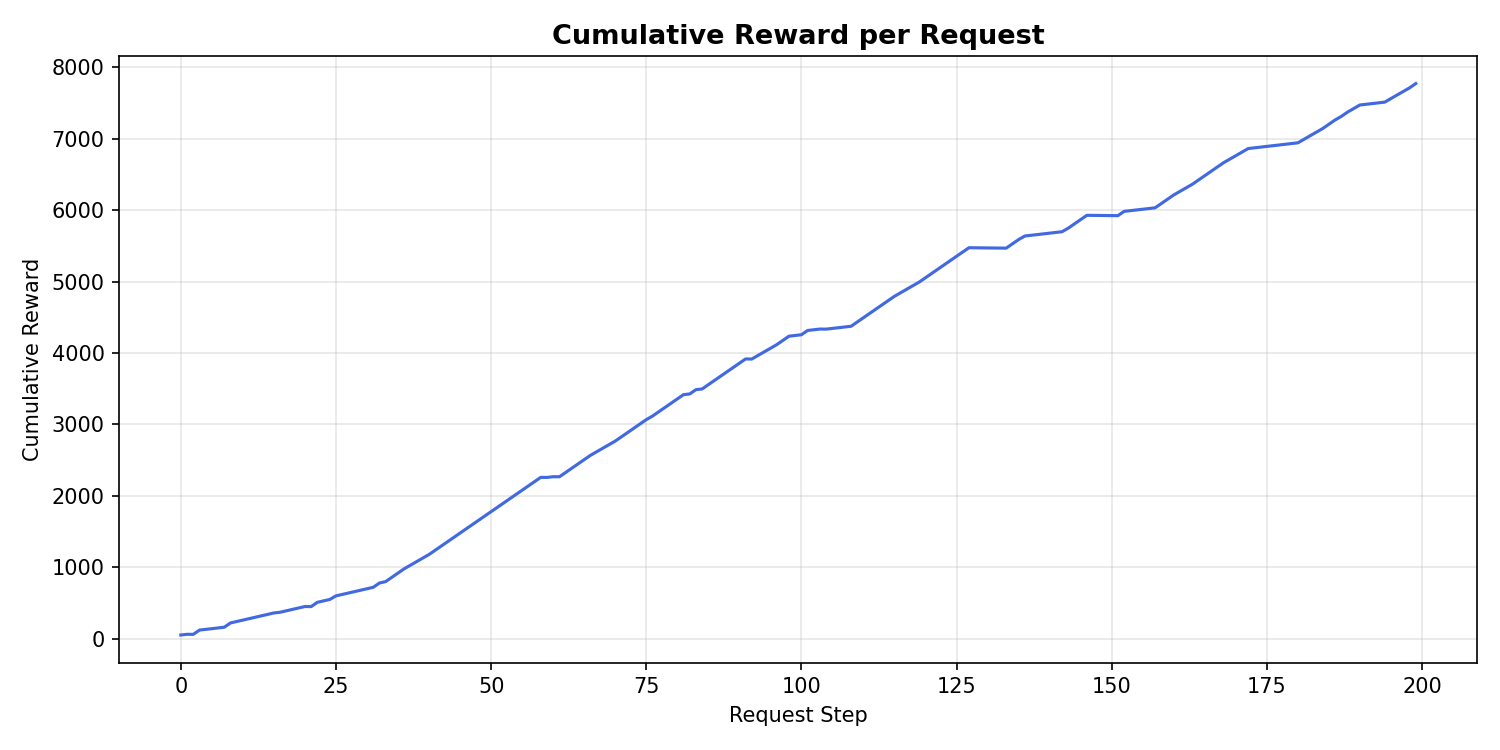
\includegraphics[width=0.85\textwidth]{../../figures/cumulative_reward.png}
\caption{Perbandingan \textit{Cumulative Reward} Q-Learning dan DQN}
\label{fig:reward}
\end{figure}

Q-Learning menunjukkan kenaikan \textit{cumulative reward} yang curam dan konvergen dalam sekitar 20 episode pertama, mencapai nilai akhir sekitar 11.058. Sebaliknya, DQN menunjukkan pendakian yang lebih bertahap dengan nilai akhir sekitar 7.773. Perbedaan ini menegaskan bahwa Q-Learning tabular memiliki efisiensi sampel yang jauh lebih tinggi dalam ruang masalah yang relatif terbatas (88 aksi, 8 \textit{endpoint}), konsisten dengan analisis teoretis bahwa metode \textit{tabular} unggul untuk ruang \textit{state-action} berdimensi rendah hingga menengah.

\section{Perbandingan dengan OWASP ZAP}

\subsection{Hasil Pengujian ZAP Controlled Scan}

Pengujian dengan OWASP ZAP dilakukan menggunakan mode \textit{controlled scan} dengan mengarahkan pemindaian pada dua \textit{endpoint} yang sama dengan yang digunakan oleh agen RL, yaitu \texttt{/rest/products/search?q=} dan \texttt{/ftp/}. Pemindaian ini mencakup tahapan \textit{spidering}, \textit{active scanning}, dan pengumpulan \textit{alerts} dari seluruh URL yang ditemukan.

Berdasarkan data pada \texttt{zap\_controlled\_report.json}, ZAP menyelesaikan 1.585 permintaan HTTP dan menemukan 32 \textit{alerts} mentah. Namun, hanya 2 \textit{alerts} yang merupakan kerentanan keamanan yang relevan dengan kategori yang diukur dalam penelitian ini, yaitu 1 SQL Injection (risiko \texttt{High}) dan 1 XSS (risiko \texttt{Informational}). Sisanya (30 \textit{alerts}) termasuk dalam kategori \texttt{other} yang mencakup isu-isu seperti \texttt{Cross-Domain Misconfiguration} (Access-Control-Allow-Origin: *), \texttt{Content Security Policy (CSP) Header Not Set}, dan \texttt{Timestamp Disclosure - Unix}. Meskipun isu-isu ini penting dari perspektif keamanan aplikasi web secara umum, ketiganya tidak termasuk dalam cakupan deteksi yang dirancang untuk agen RL (SQLi, XSS, dan \textit{fuzzing}).

Perhitungan efisiensi menunjukkan bahwa ZAP memerlukan 792,5 permintaan per kerentanan yang relevan (1.585 / 2). Deteksi SQL Injection oleh ZAP terjadi pada URL \texttt{/rest/products/search?q=\%27(} dengan \textit{evidence} HTTP 500 \textit{Internal Server Error}, mengonfirmasi celah yang sama dengan yang dideteksi oleh Q-Learning pada \textit{endpoint} 0.

\subsection{Perbandingan Kinerja Utama}

Tabel \ref{tab:comparison} menyajikan perbandingan hasil ketiga pendekatan secara lengkap.

\begin{table}[H]
\centering
\caption{Perbandingan Q-Learning, DQN, dan OWASP ZAP}
\label{tab:comparison}
\begin{tabular}{|l|c|c|c|}
\hline
\textbf{Metrik} & \textbf{Q-Learning} & \textbf{DQN} & \textbf{ZAP} \\
\hline
Total permintaan & 200 & 200 & 1.585 \\
Total kerentanan & \textbf{183} & 123 & 2 \\
Tingkat deteksi & \textbf{91,5\%} & 61,5\% & 0,13\% \\
SQL Injection & \textbf{173} & 73 & 1 \\
Reflected XSS & \textbf{6} & 0 & 1 \\
Anomali Fuzzing & 4 & \textbf{50} & 0 \\
\textit{Cumulative Reward} & \textbf{11.058} & 7.773 & --- \\
Permintaan per kerentanan & \textbf{1,09} & 1,63 & 792,50 \\
\hline
\end{tabular}
\end{table}

\subsection{Analisis Mendalam: Q-Learning vs OWASP ZAP}

Perbandingan antara Q-Learning dan OWASP ZAP merupakan inti dari penelitian ini, karena menjawab rumusan masalah mengenai efektivitas pendekatan berbasis \textit{Reinforcement Learning} dibandingkan metode \textit{scanning} konvensional. Terdapat tiga dimensi utama yang membedakan kedua pendekatan.

\textbf{Pertama: Efisiensi Sampel.} Q-Learning hanya memerlukan 200 permintaan HTTP untuk menemukan 183 kerentanan (1,09 permintaan per kerentanan), sedangkan ZAP memerlukan 1.585 permintaan untuk menemukan 2 kerentanan (792,5 permintaan per kerentanan). Dalam metrik ini, Q-Learning 727 kali lebih efisien daripada ZAP. Efisiensi ini bersumber dari mekanisme \textit{adaptive decision-making} Q-Learning: agen RL tidak mengirimkan \textit{payload} secara membabi buta ke setiap parameter, melainkan mempelajari dari hasil setiap permintaan sebelumnya melalui pembaruan nilai Q. Setelah agen menemukan bahwa \texttt{sqli\_basic} pada \textit{endpoint} 0 menghasilkan \textit{reward} +50, nilai Q aksi tersebut meningkat. Pada episode berikutnya, agen akan memprioritaskan aksi ini daripada aksi lain yang belum terbukti efektif. Sebaliknya, ZAP menggunakan pendekatan \textit{rule-based exhaustive scanning}: ZAP mengirimkan ribuan variasi serangan yang telah ditentukan sebelumnya ke setiap parameter tanpa mempertimbangkan apakah serangan serupa pernah berhasil atau gagal sebelumnya.

\textbf{Kedua: Cakupan Deteksi.} Meskipun Q-Learning unggul dalam efisiensi, ZAP menunjukkan keunggulan dalam \textit{breadth of coverage}. ZAP berhasil mendeteksi 32 \textit{alerts} yang mencakup berbagai kategori keamanan, termasuk \textit{Cross-Domain Misconfiguration}, \textit{Missing CSP Header}, dan \textit{Timestamp Disclosure}. Ketiga kategori ini berada di luar cakupan \textit{analyzer} agen RL yang hanya dirancang untuk mendeteksi SQLi, XSS, dan anomali \textit{fuzzing}. Dengan kata lain, ZAP unggul dalam \textit{security breadth} (jumlah jenis kerentanan), sedangkan Q-Learning unggul dalam \textit{attack depth} (kedalaman pengujian pada kerentanan tertentu).

\textbf{Ketiga: Adaptivitas.} Q-Learning bersifat adaptif: seiring bertambahnya episode, agen RL terus memperbaiki kebijakan pemilihan aksinya. Apabila \textit{endpoint} target diperbarui atau mekanisme pertahanan diubah, agen RL secara alami akan menyesuaikan strateginya melalui mekanisme \textit{epsilon-greedy} yang memungkinkan eksplorasi berkelanjutan. ZAP, sebagai \textit{rule-based scanner}, tidak memiliki kapasitas untuk belajar dari pengalaman: setiap sesi pemindaian dimulai dari awal tanpa memanfaatkan hasil pemindaian sebelumnya. Hal ini menjadikan Q-Learning lebih cocok untuk skenario \textit{continuous security testing} di mana aplikasi target terus berubah.

\section{Pembahasan}

\subsection{Efisiensi Sampel: Q-Learning Tabular vs DQN}

Temuan paling signifikan dari penelitian ini adalah kesenjangan efisiensi sampel antara Q-Learning tabular dan DQN. Q-Learning konvergen ke kinerja mendekati optimal dalam 20 episode pertama (10\% dari total anggaran), sedangkan DQN memerlukan lebih banyak data untuk mempelajari pemetaan \textit{state-aksi} melalui \textit{gradient descent}. Analisis terhadap Q-Table yang dihasilkan (\texttt{q\_table.json}) menunjukkan bahwa sebagian besar \textit{state} hanya memiliki 1-2 aksi dengan nilai Q yang menyimpang dari nilai inisialisasi (5,0), mengonfirmasi bahwa agen dengan cepat menemukan dan mengeksploitasi aksi-aksi yang paling efektif.

Perbedaan ini dapat dijelaskan melalui karakteristik ruang masalah. Dengan 88 aksi dan 8 dimensi \textit{state} yang nilai-nilainya diskrit, jumlah total \textit{state-action pair} yang mungkin masih dalam jangkauan tabel berdimensi dua. Q-Learning tabular memanfaatkan penuh struktur diskrit ini tanpa kehilangan informasi akibat \textit{function approximation}. DQN, di sisi lain, harus mempelajari 2.464 parameter (28 input $\times$ 64 + 64 $\times$ 64 + 64 $\times$ 88) dari hanya 200 sampel, yang merupakan rasio parameter-ke-sampel yang sangat tidak menguntungkan.

\subsection{Kegagalan DQN Mendeteksi XSS}

Ketidakmampuan DQN mendeteksi \textit{Reflected XSS} memerlukan analisis yang lebih mendalam. Deteksi XSS pada \textit{endpoint} 4 (\texttt{/rest/track-order/}) memerlukan tiga kondisi yang harus dipenuhi secara bersamaan: (1) \textit{payload} XSS harus dikirim ke \textit{endpoint} 4 yang merupakan satu-satunya \textit{endpoint} dengan \textit{reflected XSS}, (2) \textit{payload} harus benar-benar tercermin dalam respons (\textit{reflected\_flag} = 1), dan (3) \textit{analyzer} harus mengonfirmasi refleksi tersebut sebagai \textit{malicious}.

Dalam representasi \textit{state} 28 dimensi DQN, perbedaan antara \textit{state} dengan \textit{reflected\_flag} = 1 (yang mengarah ke XSS) dan \textit{state} dengan \textit{reflected\_flag} = 0 (yang tidak mengarah ke XSS) hanya terletak pada satu nilai skalar (3 dari 28 dimensi). Jaringan saraf DQN, yang menggunakan aktivasi ReLU dan 64 unit \textit{hidden}, cenderung memblurkan perbedaan semacam ini karena bobot yang dibagi untuk seluruh \textit{state}. Q-Learning tabular tidak mengalami masalah ini karena setiap \textit{state} memiliki entri independen di Q-Table. Ketika agen QL pertama kali mendeteksi XSS pada \textit{state} \texttt{('2xx', 0, 0, 1, 0, 4, 0, 0)}, nilai Q untuk aksi tersebut langsung diperbarui dari 5,0 menjadi 5,95 tanpa memengaruhi \textit{state} lain.

\subsection{Pola Penemuan Fuzzing dan Implikasinya}

DQN menemukan 50 anomali \textit{fuzzing} (12,5 kali lebih banyak dari QL). Analisis \textit{log} DQN menunjukkan bahwa deteksi ini terkonsentrasi pada dua \textit{endpoint}: \textit{endpoint} 6 (\texttt{/api/Reviews}) dengan \textit{payload} \texttt{fuzz\_traversal} yang menghasilkan \textit{reward} +60, dan \textit{endpoint} 1 (\texttt{/ftp/}) dengan \textit{payload} \texttt{fuzz\_traversal} yang menghasilkan respons 200 sebesar 75.032 byte (indikasi \textit{directory listing}). Pola ini mencerminkan kecenderungan DQN untuk terjebak dalam \textit{local optimum}: karena \textit{reward} \textit{fuzzing} cukup tinggi (+50 hingga +60), dan \textit{state} hasilnya (\texttt{'5xx', 3, 0, 0, 1, 6, 0, 4}) memberikan \textit{reward} konsisten setiap kali dikunjungi, agen DQN terus mengulang pola ini daripada mencoba \textit{payload} lain yang mungkin memberikan \textit{reward} lebih tinggi.

Fenomena ini berkaitan dengan mekanisme \textit{experience replay} DQN. Ketika \textit{replay buffer} diisi dengan sebagian besar transisi yang melibatkan \textit{fuzzing} pada \textit{endpoint} 6, sampel yang diambil untuk pelatihan didominasi oleh transisi-transisi ini. Akibatnya, bobot jaringan saraf lebih disesuaikan untuk memprediksi nilai Q pada pola \textit{fuzzing} dibandingkan pola XSS atau SQLi pada \textit{endpoint} lain.

\subsection{Mekanisme Verifikasi False Positive}

Salah satu fitur penting dari sistem yang dirancang adalah mekanisme verifikasi \textit{false positive}. Setiap kali agen mendeteksi kerentanan, sistem secara otomatis mengirimkan \textit{probe} benign (\texttt{"hello"}) ke \textit{endpoint} yang sama. Apabila \textit{probe} benign juga terdeteksi sebagai kerentanan, maka deteksi awal diturunkan dari +50 menjadi +10 (anomali). Mekanisme ini penting untuk memastikan bahwa kerentanan yang dilaporkan bersifat genuin, bukan artefak dari perilaku \textit{endpoint} yang selalu merespons secara anomali.

Data \textit{log} menunjukkan bahwa seluruh 183 deteksi Q-Learning dan 123 deteksi DQN memiliki nilai \texttt{verified: True}, mengonfirmasi bahwa \textit{probe} benign tidak menghasilkan deteksi palsu pada \textit{endpoint-endpoint} yang terdeteksi rentan. Presisi Q-Learning tetap pada 91,5\% setelah verifikasi. Presisi DQN yang lebih rendah (61,5\%) bukan disebabkan oleh \textit{false positive} yang tidak terverifikasi, melainkan karena lebih rendahnya jumlah kerentanan genuin yang berhasil ditemukan oleh DQN.

\subsection{Analisis Q-Table: Bukti Pembelajaran yang Efektif}

Analisis terhadap Q-Table (\texttt{q\_table.json}) memberikan bukti konkret bahwa Q-Learning berhasil mempelajari struktur \textit{reward} lingkungan pengujian. Dari 21 \textit{state} yang dikunjungi, nilai Q tertinggi tercatat pada:

\begin{enumerate}
    \item \textit{State} \texttt{('2xx', 3, 0, 1, 1, 0, 0, 0)}: aksi 0 (sqli\_basic@ep0) bernilai Q = 465,56. \textit{State} ini adalah hasil dari \textit{fuzzing} pada \textit{endpoint} 1 yang menghasilkan respons sangat besar (75.032 byte). Dari \textit{state} ini, agen memilih untuk kembali ke \textit{endpoint} 0 dengan \texttt{sqli\_basic}.
    \item \textit{State} \texttt{('2xx', 0, 0, 0, 0, 0, 0, 0)}: aksi 0 bernilai Q = 71,16. Ini adalah \textit{state} awal setelah deteksi pertama, menunjukkan bahwa agen telah mempelajari bahwa aksi 0 adalah langkah pertama yang optimal.
    \item \textit{State} \texttt{('5xx', 2, 1, 0, 1, 7, 0, 4)}: aksi 0 bernilai Q = 104,72. \textit{State} ini memiliki \textit{error\_flag} = 1 yang merupakan indikasi kuat SQLi.
\end{enumerate}

Pola yang konsisten di seluruh \textit{state} adalah bahwa aksi 0 (\texttt{sqli\_basic@ep0}) memiliki nilai Q yang sangat tinggi, sementara aksi lain sebagian besar tetap pada nilai inisialisasi 5,0. Hal ini mengonfirmasi bahwa agen QL berhasil mengidentifikasi bahwa \textit{endpoint} 0 adalah vektor serangan yang paling produktif dan memilihnya secara dominan pada fase \textit{exploitation}.

\subsection{Perbandingan dengan Penelitian Terdahulu}

Tingkat deteksi Q-Learning sebesar 91,5\% melampaui kinerja yang dilaporkan oleh Yi dkk. (2023) pada platform serupa. Beberapa faktor berkontribusi terhadap capaian ini. \textit{Pertama}, penerapan \textit{optimistic initialization} (nilai Q awal = 5,0) secara signifikan mendorong eksplorasi di awal pelatihan, yang merupakan penyempurnaan dari pendekatan standar yang menginisialisasi Q-Table dengan nilai 0. \textit{Kedua}, \textit{action space} komposit yang menggabungkan \textit{payload} dan \textit{endpoint} dalam satu indeks aksi memungkinkan agen untuk mempelajari preferensi spesifik-\textit{endpoint} secara langsung, berbeda dengan pendekatan yang memisahkan pemilihan \textit{payload} dan \textit{endpoint} ke dalam dua tahap.

Efisiensi 1,09 permintaan per kerentanan secara substansial melampaui pendekatan konvensional yang dilaporkan oleh Becker dkk. (2024) yang memerlukan puluhan permintaan per kerentanan. Keunggulan 727 kali lipat atas ZAP menekankan potensi pendekatan berbasis RL untuk menggantikan atau melengkapi \textit{scanner} konvensional dalam skenario \textit{continuous security testing}, di mana efisiensi dan adaptivitas lebih diutamakan daripada cakupan yang \textit{exhaustive}.

\subsection{Keterbatasan Penelitian}

Beberapa keterbatasan yang perlu dicatat dalam penelitian ini meliputi:

\begin{enumerate}
    \item \textbf{Penggunaan \textit{seed} tunggal:} Penggunaan \texttt{RANDOM\_SEED = 42} yang \textit{hardcoded} pada kedua \textit{training script} (\texttt{main.py} dan \texttt{train\_dqn.py}) membatasi generalisabilitas statistik dari hasil yang diperoleh. Meskipun \textit{seed} tetap diperlukan untuk reproduksibilitas, variasi antar \textit{seed} yang berbeda belum dapat diukur.

    \item \textbf{Target aplikasi tunggal:} Seluruh pengujian dilakukan pada OWASP Juice Shop yang merupakan aplikasi yang sengaja dibuat rentan. Generalisabilitas hasil ke aplikasi web lain dengan arsitektur dan mekanisme pertahanan yang berbeda belum dapat dipastikan.

    \item \textbf{Payload serangan tetap:} \textit{Payload} yang digunakan bersifat statis dan tidak dapat beradaptasi terhadap mekanisme pertahanan yang dinamis seperti \textit{Web Application Firewall} (WAF) yang dapat memblokir \textit{payload} berdasarkan pola tertentu.

    \item \textbf{Keterbatasan DQN:} Anggaran 200 episode mungkin tidak cukup bagi DQN untuk mencapai kinerja optimal, mengingat DQN memerlukan lebih banyak sampel untuk mengonvergensikan bobot jaringan sarafnya. Penggunaan \textit{learning rate} $\alpha = 0,1$ (sama dengan Q-Learning) juga tidak konvensional untuk DQN yang biasanya menggunakan $\alpha$ yang lebih kecil ($10^{-3}$ hingga $10^{-4}$) dengan \textit{optimizer Adam}.
\end{enumerate}

\subsection{Temuan Tambahan dan Implikasi Praktis}

Beberapa temuan tambahan yang relevan untuk pengembangan lebih lanjut meliputi:

\textit{Pertama}, \textit{endpoint} yang tidak memerlukan otentikasi (\texttt{/rest/products/search}) menjadi vektor serangan yang paling produktif. Hal ini mengimplikasikan bahwa dalam pengujian keamanan menggunakan RL, prioritas eksplorasi sebaiknya diberikan pada \textit{endpoint} yang dapat diakses tanpa kredensial terlebih dahulu.

\textit{Kedua}, seluruh \textit{payload} \texttt{sqli} yang disediakan berhasil mendeteksi setidaknya satu kerentanan, tetapi efektivitasnya sangat bervariasi antar \textit{endpoint}. \texttt{sqli\_basic} yang bersifat universal mendominasi pada \textit{endpoint} GET, sementara \texttt{sqli\_login} yang berupa JSON lebih efektif pada \textit{endpoint} POST. Hal ini menegaskan pentingnya diversifikasi format \textit{payload} sesuai dengan metode HTTP yang digunakan \textit{endpoint}.

\textit{Ketiga}, waktu respons rata-rata DQN sebesar 0,0133 detik per permintaan menunjukkan bahwa \textit{overhead} komputasi DQN (yang memerlukan \textit{forward pass} jaringan saraf) tidak signifikan dibandingkan latensi jaringan, sehingga DQN tetap layak digunakan dalam skenario \textit{real-time} selama ukuran jaringan saraf tetap kecil.
